\documentclass[a4paper,12pt]{article}
\usepackage[utf8]{inputenc}
\usepackage[T1]{fontenc}
\usepackage[spanish]{babel}
\usepackage{csquotes}
\usepackage{anysize}
\usepackage{graphicx}
\marginsize{25mm}{25mm}{25mm}{25mm}

\title{Ambiguity and the `mental eye' in pictorial relief}
\author{Jan J. Koenderink\and Andrea J. van Doorn\and Astrid M. L. Kappers}
\date{2001}

\begin{document}
{\scshape\bfseries \maketitle}

Relieve pictórico ({\itshape pictorial relief}) es un término que indica la forma de las superficies en el ``espacio pictórico'', y el espacio pictórico es la impresión espacial tridimensional obtenida cuando uno mira imágenes bidimensionales. 

Nada garantiza que aquello que creemos ver en la superficie pictórica corresponda con la realidad.

El relieve pictórico solo puede definirse de forma {\itshape operacional}. Y dada la ambigüedad inherente, no es sorprendente que distintas operacionalizaciones psicofísicas lleven a resultados distintos.

El relieve pictórico implica un estímulo, un observador y una tarea. La tarea es el instrumento para operacionalizar el relieve y para forzar una única respuesta. 

La mayor parte del trabajo hasta ahora se ha enfocado en las propiedades del estímulo --las claves de profundidad. Algunas operacionalizaciones también se han estudiado, pero sus resultados no se han comparado de forma cuantitativa. Y rara vez se ha cuantificado la influencia del sujeto --el bagaje del espectador ({\itshape beholder's share}). A menudo este bagaje es considerado un defecto y se busca reducirlo. Pero dado que la mayor parte de los estímulos especifican una escena de forma ambigua, esta no es necesariamente la mejor aproximación.

Cambiar de método cambia los resultados. Cuando dos métodos difieren en resultados se suele considerar que al menos uno de ellos está equivocado, y que un buen método reflejará la ``realidad''. Se espera que los observadores sean relativamente equivalentes y que la causa de diferencias en los juicios esté exclusivamente en los estímulos. Pero esto no parece ser el caso: la variabilidad puede provenir de los sujetos mismos.

En este estudio se comparan cuatro fonografías de esculturas abstractas en cuatro tareas con cuatro observadores. Todas las imágenes son formas genéricas de huevo con apéndices y ondulaciones menores. La mayor variación está en las tareas. Difieren con respecto al orden (profundidad u orientación de superficie), y el {\itshape scope} (muestreo local o medición global de la forma). Algunas preguntas pertinentes son
\begin{itemize}
	\item ¿El relieve se debe pensar como un mapa de la profundidad o como un arreglo de orientaciones de superficie?
	\item ¿El concepto de mapa está mal usado de inicio? ¿Debería pensarse en términos de entidades más globales?
	\item ¿Cómo manejan la ambigüedad los observadores?
\end{itemize}

{\scshape\bfseries Method}

Los observadores fueron los autores. Todos con visión corregida a la normalidad.

Los estímulos fueron fotografías monocromas digitalizadas de esculturas de Constantin Brancusi. Las esculturas se eligieron debido a que tenían forma general de huevo con variaciones menores. Todas eran parches de superficie convexos y lisos (figura 1). 

\begin{figure}[ht]
	\begin{center}
		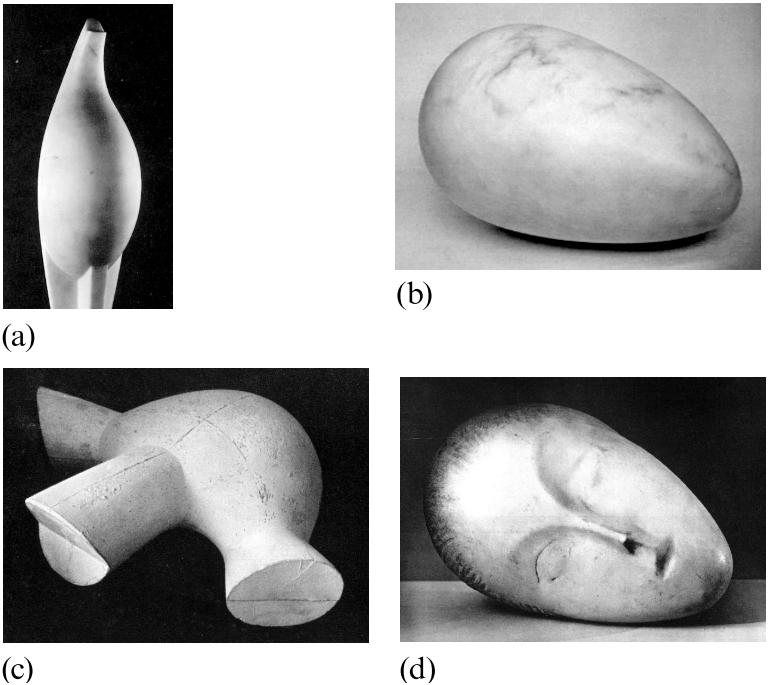
\includegraphics[scale=0.3]{Koenderick2001(1).png}
		\caption{Estímulos utilizados en la tarea.}
	\end{center}
\end{figure}

Para cada estímulo se marcó el perímetro externo y se trianguló el interior con un arreglo regular de vértices.

\begin{figure}[ht]
	\begin{center}
		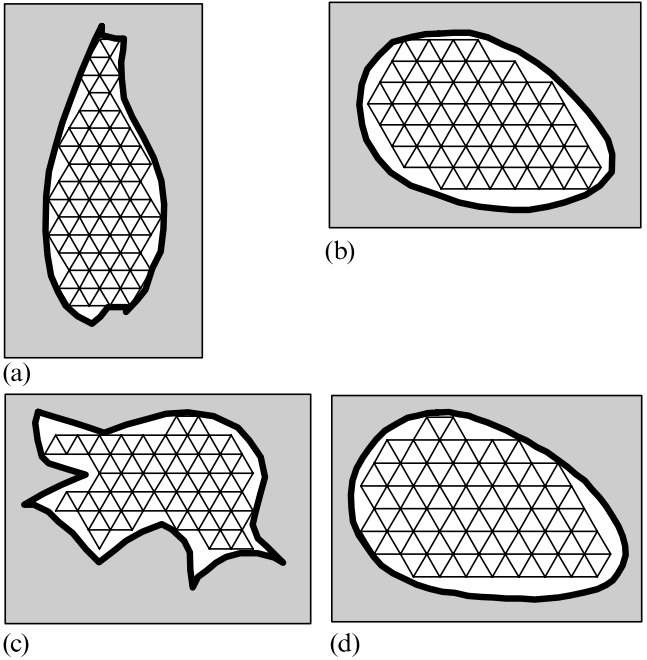
\includegraphics[scale=0.3]{Koenderick2001(2).png}
		\caption{Figuras rellenas por arreglos triangulares.}
	\end{center}
\end{figure}

Las tareas fueron ``gauge-figure adjustment'', denotada ``AT'' por {\itshape attitude probe}; ``pairwise depth difference comparison'', denotada ``PC'' por {\itshape pairwise comparison}; ``cross-secton reproduction with horizontal replica'', denotada ``CH'' por {\itshape corss-section horizontoal}; y ``cross-section reproduction with parallel replcia'', denotada ``CP'' por {\itshape cross-section parallel}. 

\begin{itemize}
	\item {\itshape Gauge-figure adjustment}: Es una tarea de sondeo de orientación de superficie local. Se superimpone una {\itshape gauge figure} roja con forma de spinner de los que salían en las papas sabritas sobre la fotografía en blanco y negro de la escultura en una ubicación aleatoria. La tarea del sujeto es variar la orientación de la {\itshape gauge figure} de modo que se vea tangente a la superficie de la escultura de la fotografía, ``como si se tratase de un círculo rojo dibujado sobre su superficie''. 
	\item {\itshape Pairwise depth-comparison}: Los puntos cuyas profundidades se deben comparar se marcan con puntos de color superpuestos sobre la fotografía en blanco y negro. El observador debe indicar cuál de los dos puntos está más cercano.
	\item {\itshape Cross-secton reproduction with horizontal replica}: Se pide a los sujetos indicar la forma de ciertos cortes de la superficie pictórica mediante el ajuste de puntos en un plano con una línea siempre horizontal (figura 3). 
	\item {\itshape Cross-section reproduction with parallel replica}. Es la misma tarea, pero en este caso la línea a ajustar era paralela a la línea dibujada sobre la superficie pictórica.
\end{itemize}

\begin{figure}[ht]
	\begin{center}
		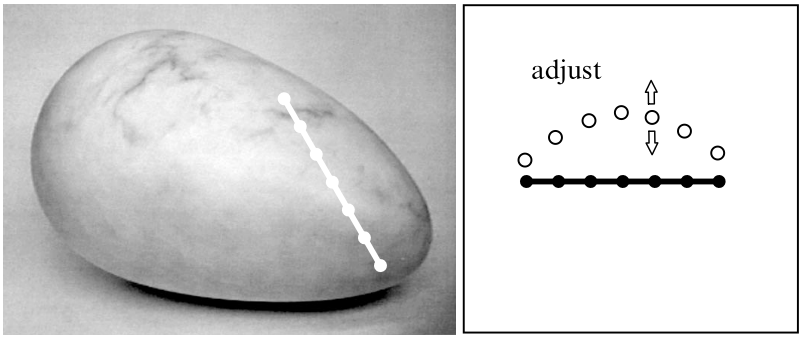
\includegraphics[scale=0.3]{Koenderick2001(3).png}
		\caption{Ilustración de la tarea 3.}
	\end{center}
\end{figure}

Todos los sujetos realizaron las cuatro tareas repetidamente para todos los estímulos. Los datos son muy ricos: en el caso de la tarea {\itshape gauge-figure} cada resultado es un par de números ({\itshape slant} y {\itshape tilt}). Para la tarea de {\itshape pairwise comparison} los resultados son booleanos.
Como una ``moneda de cambio común'' entre las tareas se convirtieron todos los resultados en un mapa de profundidades pictóricas (figura 4), pero se resalta que no se le asigna un significado especial a la profundidad sobre las otras características de las imágenes ({\itshape surface attitude} y curvatura, por ejemplo).

\begin{figure}[ht]
	\begin{center}
		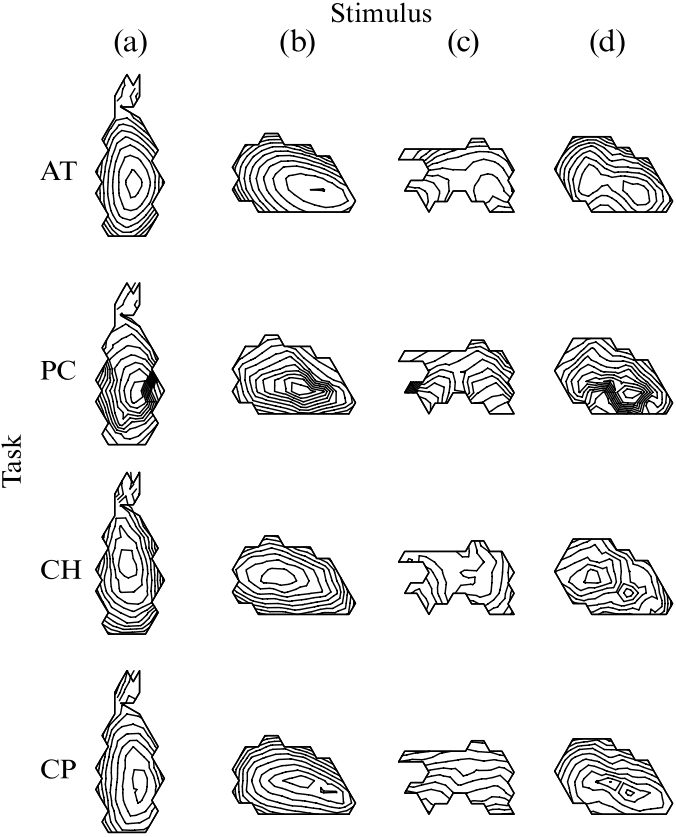
\includegraphics[scale=0.3]{Koenderick2001(4).png}
		\caption{Mapas de profundidad para cada estímulo en cada tarea de un solo sujeto.}
	\end{center}
\end{figure}

{\scshape\bfseries Analysis}

{\itshape He decidido que no me interesa el análisis y que saltaré directamente a las conclusiones. Este artículo resultó mucho menos pertinente de lo que pensaba.}

{\scshape\bfseries Conclusions}

La tarea más fácil y la que fue más ``natural'' para los sujetos fue la {\itshape gauge-figure task}. La {\itshape pairwise comparison task} es fácil también pero se siente menos natural. Las tareas {\itshape cross-section-reproduction} no son tanto ``innaturales'' como ``indirectas''. Involucran una serie de ``transformaciones mentales''.

La {\itshape gauge figure task} es la más confiables. Dado que involucra el muestreo directo de la {\itshape surface attitude} (lo que sea que eso signifique) mientras que las otras tareas implican la profundidad más directamente, se puede pensar que la representación local de la superficie es prior de un ``mapa de profundidad''.

Todas las tareas tuvieron resultados que aproximan cercanamente una superficie coherente en lugar de una nube de puntos dispersos en el espacio pictórico. 

Los relieves pictóricos son muy similares para las cuatro tareas y los cuatro observadores después de que las ambigüedades se eliminan. Esto parece indicar que distintos observadores seleccionaron el mismo conjunto de claves de profundidad y llegaron a sus percepciones de maneras similares. Se puede decir que ven espacios pictóricos tridimensionales similares cuando ven las mismas fotografías de una escena física. 

Hay importantes problemas metodológicos. Usar una regresión directa al comparar las profundidades de relieve pictórico puede llevar a concluir que los observadores no concuerdan cuando en realidad sus juicios son muy cercanos. Reportar las orientaciones locales de superficie en términos de normales de superficie no tiene sentido dado que la ortogonalidad en el espacio pictórico es destruida por la ambigüedad. 

Parece ser que los observadores aplican {\itshape scalings} y {\itshape shears} similares (quién sabe qué diablos sean), lo que indicaría que aplican priors similares. Una posible explicación para esto es que las imágenes bajodeterminan el relieve pictórico, de modo que los observadores usan la libertad restante para ajustar su {\itshape ojo mental}. Toman otra perspectiva sujeta a ciertas limitaciones. Este cambio en perspectiva puede usarse para seleccionar cualquier punto que sea localmente fronto-paralelo. 


\end{document}
